Una de las ideas más importantes obtenidas a partir del formalismo de Lagrange es la relación de las leyes de conservación con las simetrías. Se dice que un sistema es \textit{Simétrico} si bajo un sistema de transformaciones el sistema permanece invariante. 

\subsection[short]{Coordenadas cíclicas}

Cuando una coordenada generalizada no aparece de forma implícita dentro de las ecuaciones de Euler-Lagrange entonces se dice que es una $\textit{coordenada cíclica}$, por tanto, dará lugar a una constante de movimiento en el sistema. Un ejemplo, si $q^{\beta}$ no aparece dentro de la función Lagrangiana, entonces la cantidad conservada está dada por

\begin{gather*}
    \frac{d}{dt}\frac{\partial L}{\partial \dot{q}^{\beta}} = 0
\end{gather*}

Esto implica que $\partial L/ \partial \dot{q}^\beta$ será constante en el tiempo y se le da el nombre de momento conjugado generalizado $p_\beta$. Si $q^{\beta}$ es una coordenada cíclica entonces $p_\beta$ da un conjunto de sub-conjunto (sub-manifold) en $\mathbf{T}\mathbb{Q}$. Es decir, si el punto de fase inicial se encuentra en cualquier sub-conjunto cuya ecuación esta dada por $p_\beta = C$, el movimiento permanecerá en este. Todo esto implica que ahora el conjunto que contiene las ecuaciones de Euler-Lagrange es el sub-conjunto de $\mathbf{T}\mathbb{Q}$ cuya dimension  es $2n - 1$, es decir, la dimensión del colector de fase es reducida por las coordenadas cíclicas.

\subsection[short]{Transformaciones: Pasivas y Activas}

Considere una familia de transformaciones en $\mathbb{Q}$ que solo desplaza la coordenada ignorable $q^{\lambda}$ en una cantidad variable $\epsilon$. Estas transformaciones en $\mathbb{Q}$ implican otras en $\mathbf{T}\mathbb{Q}$, llamando las coordenadas transformadas como ($Q$, $\dot{Q}$), las transformaciones entre coordenadas estarán dadas por.

\begin{align*}
    Q^{\alpha} = q^{\alpha} + \epsilon\delta^{\alpha\lambda} && \dot{Q}^{\alpha} = \dot{q}^{\alpha}
\end{align*}
Donde $\delta^{\alpha\lambda}$ es la delta de Kronecker, y implica que la única coordenada que se desplaza es $q^{\lambda}$. Bajo la familia de transformaciones dadas por $\epsilon$ la función Lagrangiana se convierte en 

\begin{gather}
    \label{eq:transf}L_\epsilon(Q,\dot{Q},t) = L(q(Q,t),\dot{q}(\dot{Q},t),t)
\end{gather}
Derivando la función Lagrangiana respecto a $\epsilon$ (Esta $\epsilon$ no es la misma que se utiliza para el principio variacional), recordando que $q$ y $\dot{q}$ dependen de $\epsilon$ entonces se obtiene

\begin{gather*}
    \frac{\partial L_\epsilon}{\partial \epsilon} = \frac{\partial L}{\partial q^{\alpha}}\frac{\partial q^{\alpha}}{\partial \epsilon} + \frac{\partial L}{\partial \dot{q}^{\alpha}}\frac{\partial \dot{q}^{\alpha}}{\partial \epsilon}\\
    \frac{\partial L_\epsilon}{\partial \epsilon} = - \frac{\partial L}{\partial q^{\alpha}}\delta^{\alpha\lambda} = -\frac{\partial L}{\partial q^{\lambda}}
\end{gather*}
Como se demostró en Eq.\ref*{eq:lcova} la función $L$ es covariante ante transformación de coordenadas, entonces 

\begin{gather*}
    L_\epsilon(q,\dot{q},t) = L(q,\dot{q},t)
\end{gather*}
Esto implica
\begin{gather*}
    \frac{\partial L_\epsilon}{\partial \epsilon} = -\frac{\partial L}{\partial q^{\lambda}} = 0
\end{gather*}
Por tanto, decir que L es invariante bajo traslación en $q^{\alpha}$ es lo mismo que decir que es invariante bajo transformaciones que expresan en términos de $\epsilon$. Hay dos formas de interpretar las transformaciones dadas por la Eq.\ref*{eq:transf}. La primera interpretación es una donde el plano y todos los objetos geométricos en él permanecen fijos, pero la forma funcional del plano cambia (\textit{transformación pasiva}). La segunda interpretación el propio espacio gira, junto con todos los objetos geométricos que se encuentran en él, pero las coordenadas permanecen fijas (\textit{transformación activa}). Ambas interpretaciones se puede evidenciar en la Fig\ref*{fig:transfor}.

\begin{figure}[h]
    \centering
    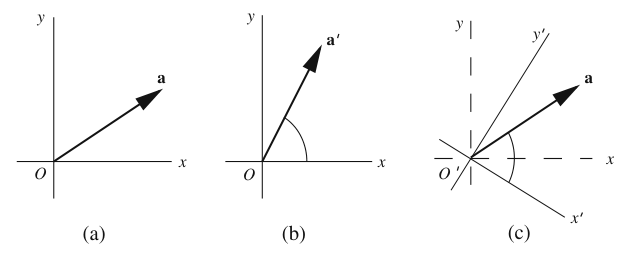
\includegraphics[scale = 1]{imgs/tps.png}
    \caption{(a) Sistema Original. (b) Transformación Activa. (c) Transformación Pasiva}
    \label{fig:transfor}
\end{figure}

\subsection[short]{Teorema de Noether}

La conexión entre la invariancia y la conservación en sistemas en los que no aparecen coordenadas ignorables esta dada mediante el \textit{Teorema de Noether}. Este teorema establece que si $L$ es invariante bajo una familia de transformaciones, su sistema dinámico posee una constante de movimiento, la cual puede ser encontrada en términos de $L$ y las transformaciones.
\vspace{2cm}
\\
Este teorema involucra familias de transformaciones continuas $\psi(\epsilon)$, dado que $L$ es una función que pertenecen a $\mathbf{T}\mathbb{Q}$ entonces es necesario estudiar las transformaciones en este espacio, esto también es debido a que transformaciones sobre $\mathbb{Q}$ implican transformaciones en $\mathbf{T}\mathbb{Q}$. Plantando una transformación pasiva, cada valor de $q$ (cada conjunto de coordenadas $q^{\alpha}$) cambia a otro $q(\epsilon)$ mediante cada valor de $\epsilon$, entonces cada trayectoria $q(t)$ cambia sus coordenadas por otras nuevas $q(t,\epsilon)$, esto permite expresar entonces a $\dot{q}(t,\epsilon)$ como  la derivada parcial de $q(t,\epsilon)$ respecto a $t$. Esto permite escribir la transformación del Lagrangiano

\begin{gather*}
    L(\xi,t) = L_\epsilon(\mathbf{T}\psi(\xi),t) 
\end{gather*}
Donde $\mathbf{T}\psi(\epsilon)$ describe una transformación en $\mathbf{T}\mathbb{Q}$ y $\xi = (q,\dot{q})$ es un punto en $\mathbf{T}\mathbb{Q}$. También es valido expresar 

\begin{gather*}
    L(q,\dot{q},t) = L\left(\psi(q),\frac{\partial \psi(q)}{\partial t},t\right)
\end{gather*}

Debido a que $L$ es covariante ante transformaciones entonces su derivada respecto a $\epsilon$ debe ser cero.

\begin{gather*}
    \frac{\partial L_\epsilon}{\partial \epsilon} = \frac{\partial L_\epsilon}{\partial q^{\alpha}}\frac{\partial q^{\alpha}}{\partial \epsilon} + \frac{\partial L_\epsilon}{\partial \dot{q}^{\alpha}}\frac{\partial \dot{q}^{\alpha}}{\partial \epsilon}  = 0
\end{gather*}
Recordando la propiedad de la Eq.\ref*{eq:prop}

\begin{gather*}
    \frac{\partial L_\epsilon}{\partial q^{\alpha}}\frac{\partial q^{\alpha}}{\partial \epsilon} + \frac{\partial L_\epsilon}{\partial \dot{q}^{\alpha}}\frac{d}{dt}\frac{\partial q^{\alpha}}{\partial \epsilon}  = 0
\end{gather*}
El segundo término de la parte izquierda se puede expresar en términos del producto de una derivada si se considera que 

\begin{gather*}
    \frac{d}{dt}\left(\frac{\partial L_\epsilon}{\partial \dot{q}^{\alpha}}\frac{\partial q^{\alpha}}{\partial \epsilon}\right) = \frac{\partial L_\epsilon}{\partial \dot{q}^{\alpha}}\frac{d}{dt}\frac{\partial q^{\alpha}}{\partial \epsilon} + \frac{\partial q^{\alpha}}{\partial \epsilon}\frac{d}{dt}\frac{\partial L_\epsilon}{\partial \dot{q}^{\alpha}}\\
    \frac{d}{dt}\left(\frac{\partial L_\epsilon}{\partial \dot{q}^{\alpha}}\frac{\partial q^{\alpha}}{\partial \epsilon}\right) - \frac{\partial q^{\alpha}}{\partial \epsilon}\frac{d}{dt}\frac{\partial L_\epsilon}{\partial \dot{q}^{\alpha}} = \frac{\partial L_\epsilon}{\partial \dot{q}^{\alpha}}\frac{d}{dt}\frac{\partial q^{\alpha}}{\partial \epsilon}
\end{gather*}
Remplazando 

\begin{gather*}
    \frac{\partial L_\epsilon}{\partial q^{\alpha}}\frac{\partial q^{\alpha}}{\partial \epsilon} + \frac{d}{dt}\left(\frac{\partial L_\epsilon}{\partial \dot{q}^{\alpha}}\frac{\partial q^{\alpha}}{\partial \epsilon}\right) - \frac{\partial q^{\alpha}}{\partial \epsilon}\frac{d}{dt}\frac{\partial L_\epsilon}{\partial \dot{q}^{\alpha}} = 0
\end{gather*}
Agrupando y remplazando la transformación $q^{\alpha} = \psi(q^{\alpha})$

\begin{gather*}
    \left(\frac{\partial L_\epsilon}{\partial q^{\alpha}} - \frac{d}{dt}\frac{\partial L_\epsilon}{\partial \dot{q}^{\alpha}} \right) \frac{\partial \psi(q^{\alpha})}{\partial \epsilon} + \frac{d}{dt}\left(\frac{\partial L_\epsilon}{\partial \dot{q}^{\alpha}}\frac{\partial \psi(q^{\alpha})}{\partial \epsilon}\right)   = 0
\end{gather*}
El primer término de esta ecuación ya es cero, debido a que son las ecuaciones de Euler-Lagrange, por lo tanto la expresión para la derivada queda expresada como

\begin{gather*}
    \frac{\partial L_\epsilon}{\partial \epsilon} = \frac{d}{dt}\left(\frac{\partial L_\epsilon}{\partial \dot{q}^{\alpha}}\frac{\partial \psi(q^{\alpha})}{\partial \epsilon}\right) 
\end{gather*}
Evaluando la derivada en $\epsilon = 0$ se obtiene su variacional, por otro lado el funcional $\psi$ siempre estará restringido por la familia de transformaciones que inicia con la transformación identidad $\psi(\epsilon = 0) = q$.

\begin{gather}
    \label{eq:vartl}\delta L_\epsilon = \frac{d}{dt}\left(\frac{\partial L_\epsilon}{\partial \dot{q}^{\alpha}}\delta q^{\alpha}\right)  = 0
\end{gather}
Esto nos indica que el argumento de la derivada será una constante de movimiento  

\begin{gather}
    \label{eq:noet}\Gamma = \frac{\partial L_\epsilon}{\partial \dot{q}^{\alpha}}\delta q^{\alpha}
\end{gather}
\\
Esto demuestra el teorema de Noether, el cual indica que si $L$ es invariante ante transformaciones puntuales (transformaciones sobre $\mathbb{Q}$), entonces existirá una constante de movimiento dada por $\Gamma$. Esto implica que a cada simetría de $L$ corresponde una constante del movimiento.\newline
Para el caso en que $L$ no se un invariante entonces la diferencia entre dos Lagrangianos es la derivada total de una función respecto al tiempo, tal como se demostró en la Eq.\ref*{eq:difl}.

\begin{gather*}
    L_\epsilon = L + \frac{d\Phi}{dt}
\end{gather*}
Donde $\Phi$ es una función de $q$, $t$ y $\epsilon$, entonces el variacional de $L$ será 

\begin{gather*}
    \delta L_\epsilon = \frac{d}{dt}\delta \Phi
\end{gather*}
Remplazando el valor de $\delta L_\epsilon$ (Eq. \ref*{eq:vartl}) se obtiene

\begin{gather*}
    \frac{d}{dt}\left(\frac{\partial L_\epsilon}{\partial \dot{q}^{\alpha}}\delta q^{\alpha}\right) = \frac{d}{dt}\delta \Phi
\end{gather*}
Por tanto, la constante de movimiento es 

\begin{gather}
    \Gamma = \frac{\partial L_\epsilon}{\partial \dot{q}^{\alpha}}\delta q^{\alpha} - \delta \Phi
\end{gather}

\subsection[short]{Ejemplo}